\documentclass[t]{beamer}
\setbeamertemplate{theorems}[numbered]
\setbeamertemplate{navigation symbols}{}
\usetheme{Frankfurt}
\usepackage{mathtext}          
\usepackage[T2A]{fontenc}          
\usepackage[utf8]{inputenc}         
\usepackage[english,russian]{babel} 
\usepackage{comment}
\newtheorem{myth}{Теорема}
\newtheorem{mylm}{Лемма}
\newtheorem*{mydef}{Определение}
\newtheorem*{mytext}{}
\newtheorem*{myco}{Следствие}
\usepackage{amsmath,amsfonts,amssymb,amsthm,mathtools}
\usepackage{icomma}
\newcommand{\pphi}[1] {P^{\delta}(\varphi_{#1})}
\usepackage{graphicx}
\hyphenpenalty=3
% \usepackage[T1]{fontenc}
% \renewcommand{\raggedright}{\leftskip=0pt \rightskip=0pt plus 0cm}
% \sloppy

\title{О длине некоторых периодических функций пятизначной логики в классе поляризованных
    полиномиальных форм}
\author{Михаил Гордеев}
\date{\today}
\institute[МГУ]{МОСКОВСКИЙ ГОСУДАРСТВЕННЫЙ УНИВЕРСИТЕТ \\
    Факультет Вычислительной Математики и Кибернетики}

\begin{document}

\frame[plain]{\titlepage}

\section{Основные определения}
\begin{frame}
\frametitle{\insertsection}
\begin{mydef}
Пусть $k \geqslant 2$ -- натуральное число, $E_k = \{0, 1, \dots, k - 1\}$.
\end{mydef}

\begin{mydef}
$f^{(n)} : E_k^n \rightarrow E_k$ называется функцией $k$-значной логики.
\end{mydef}

\begin{mydef}
$P_k^n$ -- множество всех функций $k$-значной логики, зависящих от $n$ переменных.
\end{mydef}

\begin{mydef}
Поляризованным мономом $K^{\delta}$ по вектору поляризации
$\delta = (d_1, \dots, d_n) \in E_k^n$, назовем
$(x_{i_1} + d_{i_1} )^{m_1}\cdots(x_{i_r} + d_{i_r})^{m_r}$.
\end{mydef}
\end{frame}

\begin{frame}
\frametitle{\insertsection}
\begin{mydef}
Поляризованная полиномиальная нормальная форма (ППФ) по вектору поляризации
$\delta$ -- это $\sum\limits_{i=1}^lc_i \cdot K^{\delta}_i$; $K^{\delta}_i \neq K^{\delta}_j,
i \neq j$. Число $l$ называется длиной ППФ.
\end{mydef}

\begin{mydef}
$P^{\delta}(f)$ -- это минимальная по длине, поляризованная по $\delta$ ППФ, реализующая $f$.
\end{mydef}

\begin{mydef}
$L_k(n) = \max\limits_{f\in P_k^n} \min\limits_{\delta \in E_k^n} l(P^{\delta}(f))$ -- функция
Шеннона длины.
\end{mydef}
\end{frame}

\section{Известные оценки}
\begin{frame}
\frametitle{\insertsection}
\only<1->{
\begin{mytext}
Супрун В.\,П. [1993г.], Sasao T. [1990г.] -- получили некоторые оценки для функций алгебры логики в классе
ППФ.
\end{mytext}
}
\only<2->{
\begin{mytext}
Перязев Н.\,А. [1995г.] -- 
$L_2(n) = \left[\frac{2^{n+1}}{3}\right]$.
\end{mytext}
}
\only<3->{
\begin{mytext}
Селезнева С.\,Н. [2002 г.] -- $L_k(n) < \frac{k(k-1)}{k(k-1)+1}k^n$.
\end{mytext}
}
\only<4->{
\begin{mytext}
Маркелов Н.\,К. [2012 г.] -- $L_3(n) \geqslant \left[\frac{3}{4}3^n\right]$.
\end{mytext}
}
\only<5->{
\begin{mytext}
Селезнева С.\,Н. [2015 г.] -- $L_3(n) \geqslant \left[\frac{3}{4}3^n\right]$, для симметрических
    функций.
\end{mytext}
}
\end{frame}

\section{Введение}
\begin{frame}
\frametitle{\insertsection}
\only<1>{
\begin{mydef}
Функция $k$\nobreakdash-значной логики $f(x_1 ,\dots , x_n)$ называется симметрической, если
$f(\pi(x_1), \dots, \pi(x_n)) = f(x_1, \dots, x_n)$
для произвольной перестановки $\pi$ на множестве переменных.
\end{mydef}
\begin{mydef}
Симметрическая функция $f(x_1, \dots, x_n)$ называется периодической c
периодом $\tau = (\tau_0 \tau_1 \dots \tau_{T-1}) \in E_k^T$ , если $f(\alpha) = \tau_j$ при
$|\alpha| = j\pmod T$ для каждого набора $\alpha \in E_k^n$.
\end{mydef}
}
\only<2> {
\begin{mytext}
Рассмотрим функции $f$ и $g$ -- периодические симметрические функции с периодами $(1,1,4,4)$ и
$(1,4,4,1)$ соответственно. Введем класс $\mathcal{A}$ функций вида $a \cdot f + b \cdot g$, $a,b
\in E_k$, $a \neq 0 \text{ или }b \neq 0$. И его подкласс подкласс $\mathcal{F}$ состоящий из
функций: $с \cdot f,c \cdot g,c\cdot(f+g),c \cdot (f+4g)$, $c \in \{1,2,3,4\}$.
\end{mytext}
\begin{mydef}
Пусть $T \geqslant  1$, $\Pi = \{\tau_1, \dots, \tau_s | \tau_i \in E_k^T\}$,
$A_{\Pi} = \{f_{\tau}^{(n)}|\tau \in \Pi, n \geqslant 1\}$. Класс $A_{\Pi}$ называется вырожденным,
если $\forall \tau \in \Pi$ верно, что $l(f_{\tau}^{(n)}) = \bar{o}(k^n)$, при $n\rightarrow
\infty$.
\end{mydef}
}
\end{frame}

\section{Основные теоремы и леммы}
\subsection{Длина функций $s^2$ и $s^3$}
\begin{frame}
\frametitle{\insertsection}
\framesubtitle{\insertsubsection}
\begin{myth}
\label{ths}
При $n \geqslant 1$ и $s_n$ любой из функций ${s^2_n = f_n + 2\,g_n}$, ${s^3_n = f_n + 3\,g_n}$
длина полинома периодической функции пятизначной логики~$s_n$
при поляризации $\delta = (d_1,\ldots,d_n)$выражается следующей формулой:
$$ l(P^{\delta}(s_n)) = 5^{n-m} \cdot 4^m ,$$
где $m = \begin{cases}
\text{количество } \text{ <<4>> в векторе } \delta, \text{ если } s_n = s^2_n; \\
\text{количество } \text{ <<2>> в векторе } \delta, \text{ если } s_n = s^3_n.
\end{cases}$
\end{myth}
\end{frame}

\subsection{Нижняя оценка}
\begin{frame}
\frametitle{\insertsection}
\framesubtitle{\insertsubsection}
\only<1-2> {
\begin{mylm}
При векторе поляризации $\delta = (d_1,\dots,d_n), d_i \in \{0,1,3,4\}, i = 1,\dots,n$ и
$\varphi_n$ -- любой функции из $\mathcal{F}^n$ верно:
$$l(\pphi{n}) \geqslant \frac{2}{5} \cdot 5^n.$$
\end{mylm}
}
\only<2> {
\begin{mylm}
\label{lm24l}
При векторе поляризации $\delta=(d_1,\dots,d_n),\ d_i = 2,\ i=1,\dots,m,\ d_i=4,{\ i=n-m+1,\dots,n}$
и $\varphi_n$ -- любой функции из $\mathcal{F}^n$ верно:
$$l(\pphi{n})\geqslant\left(\left(\frac{5}{4}\right)^m-\frac{3}{2}\right)\cdot4^n+4^m\cdot5^{n-m}.$$
\end{mylm}
}
\only<3> {
\begin{myth}
При векторе поляризации $\delta=(d_1,\dots,d_n)$ и $\varphi_n$ -- любой функции из
$\mathcal{F}^n$ верно: $$l(\pphi{n}) \geqslant \left(\left(\left(\frac{5}{4}\right)^{m_2}-
\frac{3}{2}\right) \cdot 4^{m_2+m_4}+4^{m_2}\cdot 5^{m_4} \right) \cdot 5^{n-m_2-m_4},$$
где $m_2$ -- число <<2>> в $\delta$, а $m_4$ -- число <<4>>.
\end{myth}
}
\end{frame}

\subsection{Верхняя оценка}
\begin{frame}
\frametitle{\insertsection}
\framesubtitle{\insertsubsection}
\only<1-2> {
\begin{myth}
\label{thh}
Для любой функции $\varphi_n$ из $\mathcal{F}^n$, при $n$ четном верно:
$$ l(\varphi_n) \leqslant 5^n\left(2\cdot\left(\frac{4}{5}\right)^{\frac{n}{2}} -
\left( \frac{4}{5} \right)^n\right).$$
\end{myth}
}
\only<2> {
\begin{myco}
Класс функций $\mathcal{A}$ является вырожденным.
\end{myco}
}
\end{frame}

\section{Результаты}
\subsection{Математические результаты}
\begin{frame}
\frametitle{\insertsection}
\framesubtitle{\insertsubsection}
\begin{enumerate}
\item Для всех функций из класса $\mathcal{A}$ были построены построены все поляризованные
полиномы, выражающие функции от $n+1$ переменных через функции от $n$ переменных также принадлежащих
классу $\mathcal{A}$;
\item<2-> Установле точная длина, в зависимости от поляризации, для функций: $s^2_n$ и $s^3_n$;
\item<3-> Доказано несколько теорем и лемм, из которых получается нижняя оценка для функций из
класса $\mathcal{F}$;
\item<4-> Установлена верняя оценка для функций из класса $\mathcal{F}$;
\item<5-> Доказана вырожденность класса $\mathcal{A}$.
\end{enumerate}
\end{frame}

\subsection{Программные результаты}
\begin{frame}
Для получения результатов были написаны следующие программы:
\frametitle{\insertsection}
\framesubtitle{\insertsubsection}
\only<1> {
\begin{itemize}
\item Программа на языке {\ttfamily{C++}}, реализующая построение поляризованных полиномов по
    модулю~$k$, где $k \in {2,3,5,7}$;
\item Для этой программы был написан интерфейс на языке {\ttfamily{Perl}}, передставленный на
    рисунке;
    \begin{figure}[h]
    \centering
    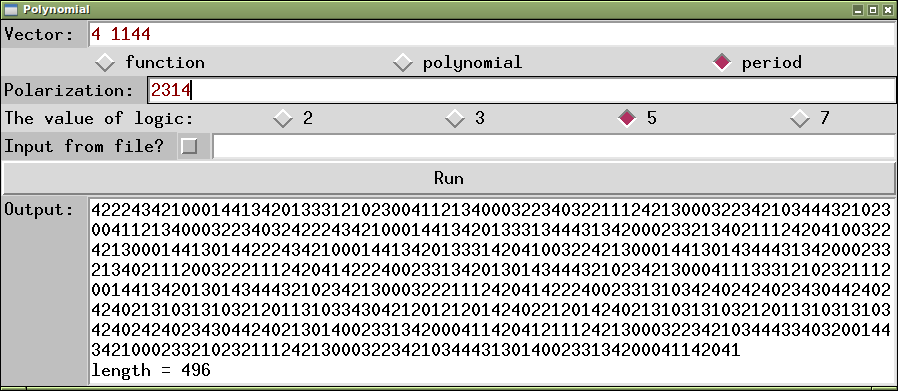
\includegraphics[width=0.65\textwidth]{polyscreen.png}
    \end{figure}
\end{itemize}
}
\only<2> {
\begin{itemize}
\item Программа на языке {\ttfamily{C++}}, осуществляющая для заданного числа пременных $n$
    "быстрый"{} поиск функций длина которых, в классе пляризованных полиномов, больше заданного
    порога, среди заданного класса симметрических функций от $n$ переменных;
\item С помощью системы компьютерной алгебры {\ttfamily{Sage}} были произведены: получение
    полиномиальных форм, поляризованных по разным векторам поляризации и подстановка значений в
    полиномы для проверки правильности их построения.
\end{itemize}
}
\end{frame}

\section*{}
\begin{frame}[plain,c]
\begin{center}
\Huge Спасибо за внимание
\end{center}
\end{frame}

\end{document}
